\mode*
\part{Shell Basics}
\lecture{shell}{shell}

\section{Shell Basics}
\label{sec:basic-commands}

\begin{frame}{Shell}
  \begin{itemize}
  \item[\shell] A command line interpreter
  \item[\shell] A programming language
  \end{itemize}
  \begin{center}
    \mode<beamer>{ 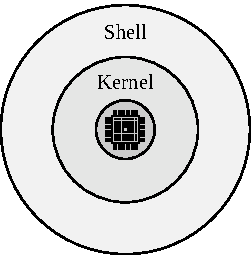
\includegraphics[width=.5\textwidth]{sys-arch} }%
    \mode<article>{ 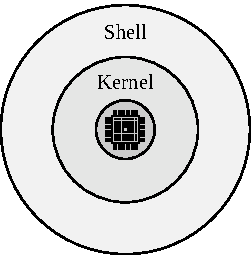
\includegraphics[width=.2\textwidth]{sys-arch} }
  \end{center}
\end{frame}

\begin{frame}{Directory Structure}
  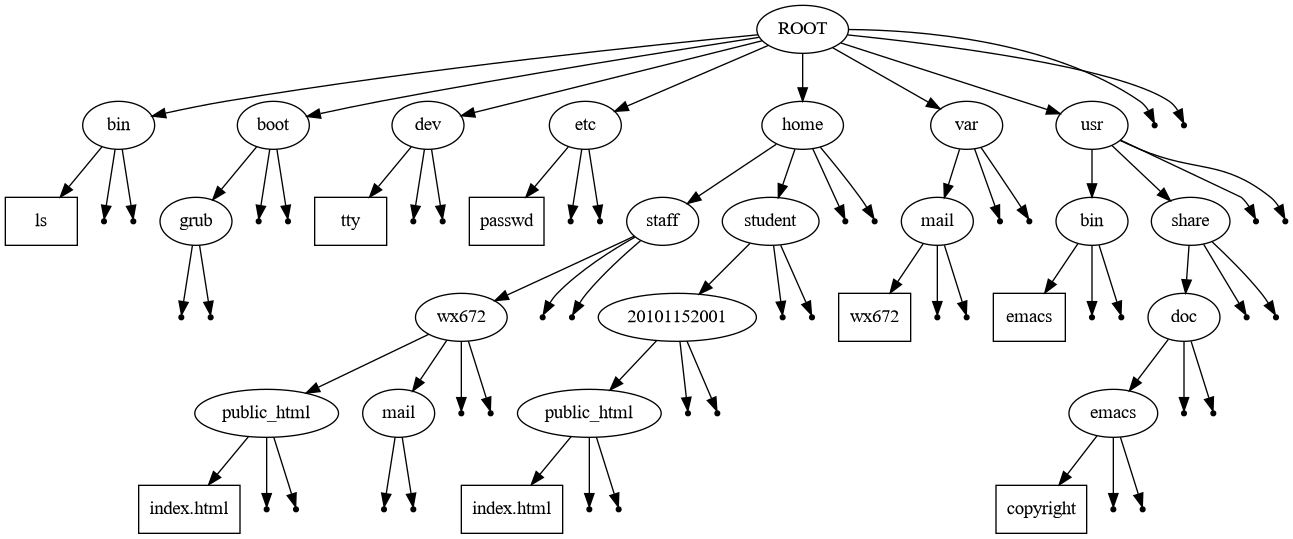
\includegraphics[width=\linewidth]{cs2}
  
  \begin{center}\small
    \begin{tabular}{r@{\qquad}>{\ttfamily}l}
      \hline
      \thead{Todo}  & \thead{How}  \\\hline
      Where am I?   & pwd          \\
      What's in it? & ls           \\
      Move around?  & cd           \\
      Disk usage?   & du, df       \\
      USB drive?    & lsblk, mount \\
      New folder?   & mkdir        \\
      \hline
    \end{tabular}
  \end{center}
\end{frame}

\begin{frame}{File Operations}
  \begin{iblock}{Ways to create a file}
    \begin{itemize}
    \item[\vim] Using an editor (vim, emacs, nano\ldots), or
    \item[\$] \cmd{cat > filename}
    \item[\$] \cmd{echo "hello, world" > filename}
    \item[\$] \cmd{touch filename}
    \end{itemize}
  \end{iblock}
  More file operations:
  \begin{center}\small
    \begin{tabular}{r@{\quad}>{\ttfamily}l|r@{\quad}>{\ttfamily}l}
      \hline
      \thead{Todo} & \thead{How} & \thead{Todo} & \thead{How}         \\\hline
      Copy?        & cp          & Move/Rename? & mv                  \\
      Delete?      & rm          & What's it?   & file                \\
      Link?        & ln          & Permission?  & chmod, chown        \\
      Count?       & wc          & Archive?   & tar, gzip, 7z, \ldots \\
      Sort?        & sort, uniq  & Search?      & find, grep          \\
      \hline
    \end{tabular}
  \end{center}
\end{frame}

\begin{frame}{Redirection}
  \begin{iblock}{Redirecting output}\ttfamily
    \begin{itemize}
    \item[\$] ls -l > output.txt
    \item[\$] ps aux >> output.txt
    \end{itemize}
  \end{iblock}
  \begin{iblock}{Redirecting input}\ttfamily
    \begin{itemize}
    \item[\$] more < output.txt
    \end{itemize}
  \end{iblock}
\end{frame}

\begin{frame}{Process Operations}
  \begin{center}\small
    \begin{tabular}{r@{\quad}>{\ttfamily}l|r@{\quad}>{\ttfamily}l}
      \hline
      \thead{Todo} & \thead{How} & \thead{Todo} & \thead{How}         \\\hline
      Kill?&kill, Ctrl-c&suspend?&Ctrl-z\\
      background?&bg, \& &forground?&fg, jobs\\
      status?&ps, top&&\\\hline
    \end{tabular}
  \end{center}
\end{frame}

\begin{frame}{System Info}
  \begin{center}\small
    \begin{tabular}{r@{\quad}>{\ttfamily}l|r@{\quad}>{\ttfamily}l}
      \hline
      \thead{Todo}   & \thead{How}         & \thead{Todo} & \thead{How}  \\\hline
      who?           & w, who, whoami      & how long?    & uptime       \\
      software?      & apt, aptitude, dpkg & kernel?      & uname, lsmod \\
      hardware?      & lspci, lsusb, lscpu & memory?      & free, lsmem  \\\hline
    \end{tabular}
  \end{center}
  \begin{block}{APT --- ~\debian~package management}
    \begin{center}\small
      \begin{tabular}{l>{\ttfamily}l}
        \hline
        \thead{Todo} & \thead{How}                                       \\\hline
        upgrading?   & apt update \&\& apt upgrade                       \\
        install?     & apt install xxx                                   \\
        remove?      & apt purge xxx                                     \\
        search?      & apt search xxx                                    \\
        details?     & apt show xxx                                      \\
        friendly UI? & aptitude                                          \\\hline
      \end{tabular}
    \end{center}
  \end{block}
\end{frame}

\begin{frame}{CLI Shortcuts}
  \begin{center}
    \begin{tabular}{>{\ttfamily}r@{\quad}l|>{\ttfamily}r@{\quad}l}
      \Ca: & beginning of line  & \Ce:  & end of line      \\
      \Cf: & forward            & \Cb:  & backward         \\
      \Cn: & next               & \Cp:  & previous         \\
      \Cr: & reverse search     & \Cu:  & cut to beginning \\
      \Ck: & kill (cut to end)  & \Cy:  & yank (paste)     \\
      \Cd: & delete a character & \Tab: & completion       \\
    \end{tabular}
  \end{center}
  \begin{block}{Tmux}
    \begin{center}
    \begin{tabular}{>{\ttfamily}r@{\quad}l|>{\ttfamily}r@{\quad}l}
      \Ca {\kbd c}:  & create window      & \Ca \Ca: & switch window    \\
      \Ca {\kbd n}:  & next window        & \Ca {\kbd p}:   & previous window  \\
      \Ca {\kbd -}:  & split window       & \Ca {\kbd |}:   & split widnow     \\
      \Ca {\kbd j}:  & go down            & \Ca {\kbd k}:   & go up            \\
      \Ca {\kbd l}:  & go right           & \Ca {\kbd h}:   & go left          \\
    \end{tabular}
    \end{center}
  \end{block}
\end{frame}

\begin{frame}{Understanding ``\texttt{ls -l}''}
  \begin{minipage}{.71\linewidth}
    \begin{center}
      \mode<beamer>{ 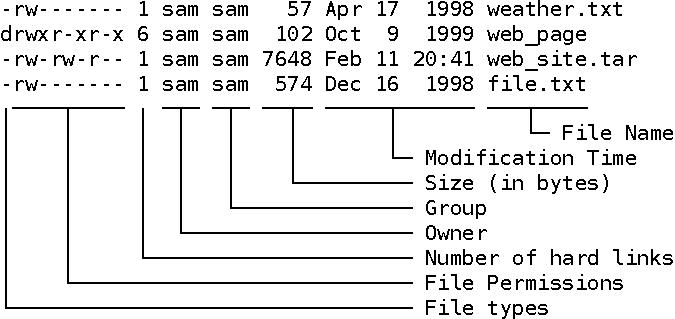
\includegraphics[width=\textwidth]{ls-l} }%
      \mode<article>{ 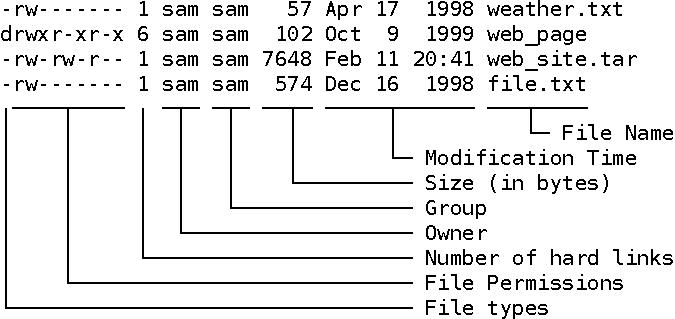
\includegraphics[width=.7\textwidth]{ls-l} }
    \end{center}
  \end{minipage}\quad
  \begin{minipage}{.25\linewidth}\scriptsize
    \begin{tabular}{c@{\;-\;}l}
      d& directory\\
      -& regular file\\
      l& soft link\\
      c& character device\\
      b& block device\\
      s& socket\\
      p& named pipe (FIFO)
      \end{tabular}
  \end{minipage}

  \begin{iblock}{9-bit permission}
    \begin{minipage}{.27\linewidth}
      \begin{center}
        \mode<beamer>{ 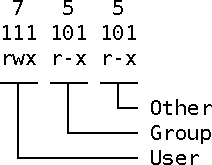
\includegraphics[width=\textwidth]{9bit} }%
        \mode<article>{ 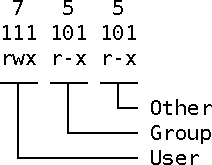
\includegraphics[width=.6\textwidth]{9bit} }
      \end{center}
    \end{minipage}\quad
    \begin{minipage}{.5\linewidth}\small
      \begin{tabular}{l@{\qquad}l}
        \CMD{chmod 755 foo}&\CMD{chmod 644 foo}\\
        \CMD{chmod 000 foo}&\CMD{chmod 777 foo}\\
        \CMD{chmod a-r foo}&\CMD{chmod u+x foo}\\
        \CMD{chmod g+w foo}&\CMD{chmod go=rx foo}
      \end{tabular}
    \end{minipage}
  \end{iblock}
\end{frame}

\begin{frame}{Wildcard Expansion}
  \begin{center}
    \begin{tabular}{>{\ttfamily}rl>{\ttfamily}l}
      \hline
      \thead{Character}&\thead{Meaning}&\thead{Example}\\\hline
      ?&any one&\CMD{ls ???.txt}\\
      *&zero or more&\CMD{ls *.c}\\
      {[]}&or&\CMD{ls *.[ch]}\\
      \{\}&and&\CMD{ls *.\{c,h,cpp\}}\\\hline    
    \end{tabular}
  \end{center}
  \begin{iblock}{Example}
    \CMD{touch \{2,3,4,234\}.\{jpg,png\} \&\& ls}\\[1ex]
    \begin{description}
    \item[output:]
      \begin{tabular}{*{4}{>{\ttfamily}r}}\hline
        2.jpg&234.jpg&3.jpg&4.jpg\\
        2.png&234.png&3.png&4.png\\\hline
      \end{tabular}
    \end{description}
    \vspace*{1ex}
    \begin{multicols}{2}
      \begin{itemize}
      \item[\$] \cmd{rm [234].jpg}
      \item[\$] \cmd{rm \{2,3,4,234\}.jpg}
      \item[\$] \cmd{rm 2*}
      \item[\$] \cmd{rm ?.jpg}
      \item[\$] \cmd{rm ?.*}
      \item[\$] \cmd{rm *}
      \end{itemize}
    \end{multicols}
  \end{iblock}
\end{frame}

\begin{frame}{Everything Is A File}
  \begin{itemize}
  \item[\$] \cmd{cat /dev/null > /var/log/messages \# empty a file}
    \begin{itemize}
    \item[\$] \cmd{: > /var/log/messages \# no new process}
    \end{itemize}
  \item[\$] \cmd{ls > /dev/null}
  \item[\$] \cmd{dd if=/dev/zero of=/tmp/clean bs=1k count=1k}
  \item[\$] \cmd{dd if=/dev/urandom of=/tmp/random bs=1k count=1k}
  \end{itemize}
\end{frame}

\begin{frame}{\texttt{/proc}}
  Allow higher-level access to driver and kernel information
  \ttfamily
  \begin{itemize}
  \item[\$] cat /proc/cpuinfo
  \item[\$] cat /proc/meminfo
  \item[\$] cat /proc/version
  \item[\$] cat /proc/1/status
  \item[\#] echo 100000 > /proc/sys/kernel/pid\_max
  \end{itemize}
\end{frame}

\begin{frame}{Pipe --- Chain Processes Together}
  \begin{itemize}
  \item[\$] \cmd{ls | wc -l}
  \end{itemize}
  \begin{center}
    \mode<beamer>{ 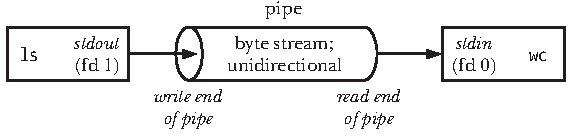
\includegraphics[width=.7\textwidth]{pipe-ls-wc} }%
    \mode<article>{ 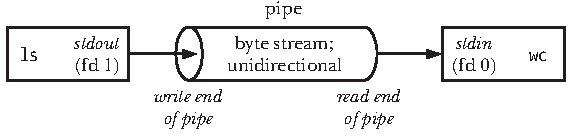
\includegraphics[width=.6\textwidth]{pipe-ls-wc} }
  \end{center}
  \begin{description}
  \item[Unnamed pipe] \,\\
    \CMD{unicode skull | head -1 | cut -f1 -d' ' | sm -}
  \item[Named pipe] \,\\
    \begin{enumerate}
    \item \CMD{mkfifo mypipe}
    \item \CMD{gzip -9 -c < mypipe > out.gz}
    \item \CMD{cat file > mypipe}
    \end{enumerate}
  \end{description}
\end{frame}

\begin{itemize}
\item \url{https://en.wikipedia.org/wiki/Named_pipe}
\end{itemize}

\section{Shell Programming}
\label{sec:shell-programming}

\begin{frame}{\$ --- Give Me The Value Of \ldots}
  \begin{description}
  \item[\texttt{\$var}] Give me the value of variable ``\texttt{var}''
  \item[\texttt{\$(echo hello)}] Give me the value (output) of command ``\cmd{echo hello}''
  \item[\texttt{\$((1+1))}] Give me the value (result) of ``1+1''
  \item[\texttt{\$\$}] Give me the value of special variable ``\texttt{\$}''
  \item[\texttt{\$?}] Give me the value of special variable ``\texttt{?}''
  \item[\texttt{\$0}] Give me the value of special variable ``\texttt{0}''
  \item[\texttt{\$@}] Give me the value of special variable ``\texttt{@}''
  \end{description}
\end{frame}

\begin{frame}{Variables}\ttfamily\small
  \begin{itemize}
  \item[\$] a=8; b=2
  \item[\$] a=a+5; a=\$a+5 \Bad
  \item[\$] let a=a+5; let a+=5; a=\$((a+5)) \Good
  \item[\$] let b=b+a; let b+=a; b=\$((b+a)) \Good
  \item[\$] echo a; echo \$a
  \item[\$] (( a=5, b=6, a+=b )) \Good
  \item[\$] (( b = a<5 ? 8 : 9 )) \Good
  \item[\$] r=\$(( RANDOM\%100 )) \Good
  \item[\$] echo "\$a" \# partial quoting
  \item[\$] echo '\$a' \# full quoting
  \item[\$] a=\$(ls -l); echo \$a; echo "\$a"
  \item[\$] a=hello; b=world; let a+=b \Bad
  \end{itemize}
\end{frame}

\begin{frame}{Positional Parameters}{\cmd{\$0, \$1, \$2, \ldots, \$@, \$\#}}
  \begin{minipage}{.44\linewidth}
    \begin{center}
      \mode<beamer>{ 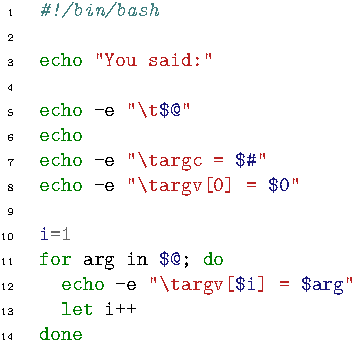
\includegraphics[width=\textwidth]{isay-sh} }%
      \mode<article>{\shellfile{../src/isay.sh}}
    \end{center}
  \end{minipage}\quad
  \begin{minipage}{.52\linewidth}
    \begin{center}
      \mode<beamer>{ 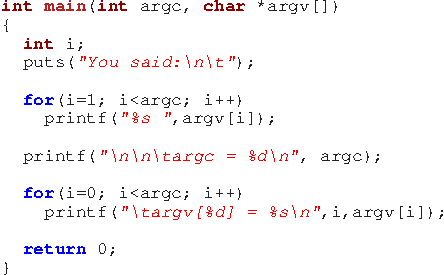
\includegraphics[width=\textwidth]{isay-c} }%
      \mode<article>{\cfile{../src/isay.c}}
    \end{center}
  \end{minipage}
\end{frame}

\begin{frame}{Parameter Substitution}
  \begin{iblock}{Default value}\ttfamily
    \begin{multicols}{2}
      \begin{itemize}
      \item[\$] echo \$\{s:=abc\}
      \item[\$] echo \$\{s:=xyz\}
      \item[\$] echo \$\{v:-8\}
      \item[\$] echo \$\{v:-10\}
      \end{itemize}
    \end{multicols}
  \end{iblock}
  \begin{iblock}{Example}
    \begin{center}
      \mode<beamer>{ 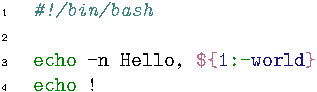
\includegraphics[width=.6\textwidth]{para-substitution-sh} }%
      \mode<article>{\shellfile{../src/para-substitution.sh}}
    \end{center}
  \end{iblock}
  \begin{itemize}
  \item[\hw] Re-write it in C
  \end{itemize}
\end{frame}
\begin{itemize}
\item[\$] \cmd{sudo apt install abs-guide}
\item \url{file:///usr/share/doc/abs-guide/html/parameter-substitution.html}
\end{itemize}

\begin{frame}{Parameter Substitution}
  \begin{iblock}{Substring removal}
    \CMD{for f in *.pbm; do ppm2tiff \$f \$\{f\%pbm\}tif; done}
  \end{iblock}
  \begin{iblock}{Substring replacement}
    \CMD{for f in *.jpg; do mv \$f \$\{f/jpg/JPG\}; done}
  \end{iblock}  
\end{frame}

\begin{frame}{Environmental Variables}\ttfamily
  \begin{iblock}{Each process has an environment}
    \begin{center}\small
      \begin{tabular}{lllll}
        \$PATH&\$PWD&\$HOME&\$UID&\$USER\\
        \$GROUPS&\$SHELL&\$TERM&\$DISPLAY&\$TEMP\\
        \$HOSTNAME&\$HOSTTYPE&\$IFS&\$EDITOR&\$BROWSER\\
        \$HISTSIZE&\$FUNCNAME&\$TMOUT&\ldots&\\
      \end{tabular}
    \end{center}
    \begin{itemize}
    \item[\$] export HISTSIZE=2000
    \item[\$] export BROWSER='/usr/bin/x-www-browser'
    \item[\$] export EDITOR='vim'
    \item[\$] export ALTERNATE\_EDITOR="vim"
    \item[\$] export PDFVIEWER='/usr/bin/zathura'
    \end{itemize}
  \end{iblock}
  \begin{itemize}
  \item[\$] env
  \item[\$] declare
  \end{itemize}
\end{frame}

\begin{frame}[allowframebreaks]{Tests}\small\ttfamily
  \begin{itemize}
  \item[\$] (( 5 < 6 )) \&\& echo should be
  \item[\$] [[ 1 < 2 ]] \&\& echo of course
  \item[\$] [[ \$a -lt \$b ]] \&\& echo yes || echo no
  \item[\$] if [[ \$a -lt \$b ]]; then echo yes; else echo no; fi
  \item[\$] if test \$a -lt \$b; then echo of course; fi
  \item[\$] if test \$a = 5; then echo a=\$a; fi \correct
  \item[\$] if test a = 5; then echo a=\$a; fi \wrong
  \item[\$] if test a=5; then echo a=\$a; fi \Bad{} \# test ls,cd,\ldots
  \item[\$] if a = 5; then echo a=\$a; fi \wrong{} \# whitespace matters
  \item[\$] if a=5; then echo a=\$a; fi \Okay
  \item[\$] test \$a = 5 \&\& echo a=\$a \correct
  \item[\$] [[ \$a = 5 ]] \&\& echo a=\$a \correct
  \item[\$] if cmp a b; then echo same file; fi \correct
  \item[\$] [[ cmp a b ]] \&\& echo same file \wrong
  \item[\$] if test cmp a b; then echo same file; fi \wrong
  \item[\$] [[ -f \symbol{`~}/.bash\_aliases ]] \&\& . \symbol{`~}/.bash\_aliases
  \item[\$] [[ -x /usr/bin/xterm ]] \&\& /usr/bin/xterm -e tmux \&
  \item[\$] [[ "\$pass" != "\$MYPASS" ]] \&\& echo 'Wrong password!' \&\& exit 1
  \item[\$] help test
  \end{itemize}
  \begin{iblock}{}
    \begin{center}
      \mode<beamer>{ 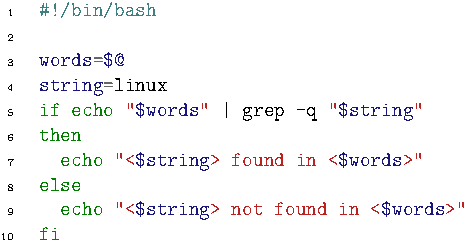
\includegraphics[width=.7\textwidth]{if-then-else-sh} }%
      \mode<article>{\shellfile{../src/if-then-else.sh}}
    \end{center}
  \end{iblock}
\end{frame}

\begin{frame}{Loops}{\ttfamily for ARG in LIST; do COMMAND(s); done}\small\ttfamily
\begin{itemize}
\item[\$] for i in 1 2 3; do echo -n i="\$i "; done
\item[\$] for i in \{1..10\}; do echo \$i; done
\item[\$] for i in \$(seq 10); do echo \$i; done
\item[\$] for ((i=1; i<=10; i++)); do echo \$i; done
\item[\$] for ((i=1, j=1; i<=10; i++, j++)); do\\
  \quad{}echo \$((i-j)) \Good\\
  \quad{}echo \$((\$i-\$j)) \Good\\
  \quad{}echo \$i-\$j \Bad\\
  done
\item[\$] for ((i=1; i<=10; i++)) \{ echo \$i; \} \# C style
\item[\$] for i in hello world; do echo -n "\$i "; done
\end{itemize}
\end{frame}

\begin{frame}{Loops}{\ttfamily while CONDITION; do COMMAND(s); done}\small\ttfamily
\begin{itemize}
\item[\$] a=0; 
\item[\$] while [[ \$a -lt 10 ]]; do echo \$a; ((a++)); done \correct
\item[\$] while \ [ \$a -lt 10 ] ; do echo \$a; ((a++)); done \correct
\item[\$] while [[ \ a < 10 ]]; do echo \$a; ((a++)); done \wrong
\item[\$] while [[ \$a < 10 ]]; do echo \$a; ((a++)); done \wrong
\item[\$] while (( a < 10 )) ; do echo \$a; ((a++)); done \correct
\item[\$] until (( a == 10 )); do echo \$a; ((a++)); done \correct
\item[\$] until (( a = 10 )) ; do echo \$a; ((a++)); done \Bad
\item[\$] while read n; do n2 \$n; done
\item[\$] while read n; do n2 \$n; done < datafile
\item[\$] until (( n == 0 )); do read n; n2 \$n; done
\end{itemize}
\end{frame}

\begin{frame}{\texttt{case}}
  \begin{center}
    \mode<beamer>{ 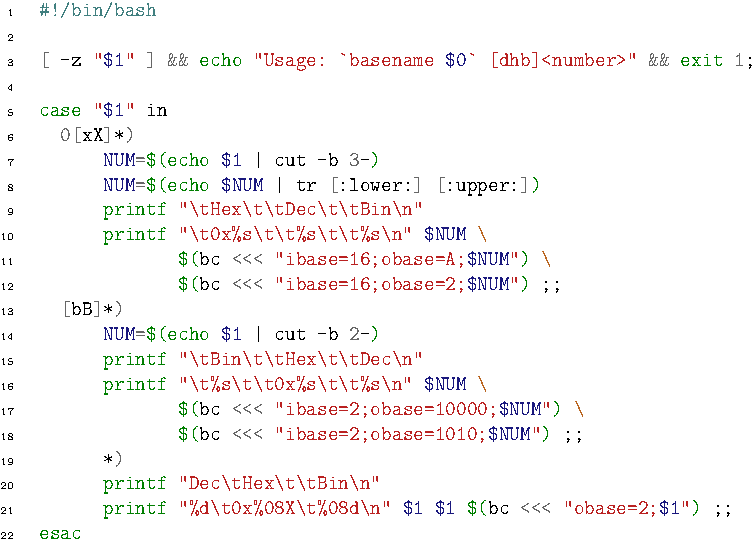
\includegraphics[width=.8\textwidth]{n2-sh} }%
    \mode<article>{\shellfile{../src/n2.sh}}
  \end{center}
\end{frame}

\begin{frame}{\texttt{select}}
  \begin{center}
    \mode<beamer>{ \includegraphics[width=\textwidth]{select-sh} }%
    \mode<article>{\shellfile{../src/select.sh}}
  \end{center}
\end{frame}

\begin{frame}{Functions}
  \mode<beamer>{ \includegraphics[width=\textwidth]{func-sh} }%
  \mode<article>{\shellfile{../src/func.sh}}
\end{frame}

\begin{frame}{Array}
  \begin{center}
    \mode<beamer>{ 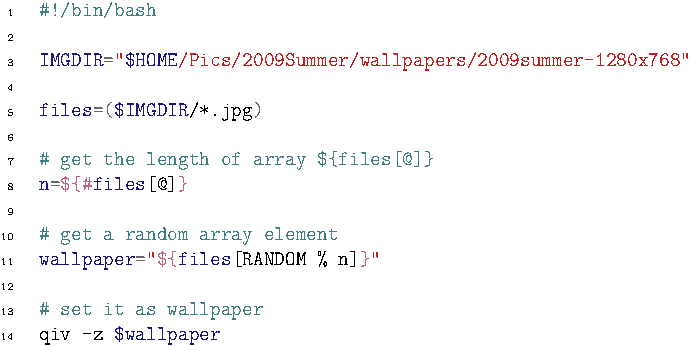
\includegraphics[width=\textwidth]{wallpaper-sh} }%
    \mode<article>{\shellfile{../src/wallpaper.sh}}
  \end{center}
  \begin{itemize}
  \item[\hw] Change wallpaper every 5 mins?
  \end{itemize}
\end{frame}

\begin{itemize}
\item \url{https://www.tutorialspoint.com/unix/unix-using-arrays.htm}
\end{itemize}

\begin{frame}{Subshells}\ttfamily
  \begin{itemize}
  \item[\$] read first second\\
    \quad hello world
  \item[\$] echo \$first \$second
  \item[] 
  \item[\$] read first second <<<'hello world'
  \item[\$] echo \$first \$second
  \end{itemize}
  \begin{iblock}{Subshell examples}
    \begin{itemize}
    \item[\$] echo hello world | (read f s; echo \$f \$s)
    \item[\$] echo \$f \$s
    \item[] 
    \item[\$] x=out; (x=in; echo \$x)
    \end{itemize}
  \end{iblock}
\end{frame}

\begin{itemize}
\item \url{file:///usr/share/doc/abs-guide/html/subshells.html}
\item \url{file:///usr/share/doc/abs-guide/html/process-sub.html}
\end{itemize}



\mode<all>
%%% Local Variables:
%%% mode: latex
%%% TeX-master: "lap-b"
%%% End:
